%!TeX program = xelatex
%Do not change
\documentclass[12pt, oneside]{article}
\usepackage{amssymb,amsmath}
\usepackage[margin=1in]{geometry}
\usepackage{textpos}
\usepackage{float}
\usepackage{booktabs}
%\usepackage{color}
\usepackage{graphicx}
\usepackage[inter-unit-product =\cdot]{siunitx}
\let\DeclareUSUnit\DeclareSIUnit
\let\US\SI
\DeclareUSUnit\inch{in}
\DeclareUSUnit\foot{ft}
\DeclareUSUnit\mile{mi}
\DeclareUSUnit\foot{ft}
\DeclareUSUnit\slug{slug}
\DeclareUSUnit\pound{lb}
\DeclareUSUnit\psi{psi}
\DeclareUSUnit\Msi{Msi}
\DeclareUSUnit\ksi{ksi}

%\usepackage{tikz}
%\usetikzlibrary{positioning}
%\usepackage{tikz-3dplot}
%\usepackage{pgfopts}
%\usepackage{wasysym}
%\usepackage{stanli}

% You may add the packages you need here
\begin{document}

%TODO change numbers in problems
\begin{textblock*}{4cm}(-1.7cm,-2.3cm)
\noindent {\scriptsize AE333 Fall 2020}
\end{textblock*}

%Do not modify other than putting your name where stated
\begin{textblock*}{8cm}(12.5cm,-1cm)
\noindent {Name: }
\end{textblock*}
%Do not modify other than typing your acknowledgement where stated
\begin{textblock*}{13.5cm}(-1.7cm,-1.8cm)
%\noindent \textit{\footnotesize Acknowledgement: Your acknowledgement for collaboration and other sources goes here. }
\end{textblock*}

\vspace{1cm}

%Do not modify other than typing the homework number after #
\begin{center}
\textbf{\Large Homework 9 Solutions}

\textbf{Due 10 November 2020}
\end{center}

\begin{enumerate}
	\item %12-6
		Find the deflection (as a function of $x$) for a cantilevered beam with an applied end moment.
		Assume $EI$ is constant and express answer in terms of applied moment and $EI$.
		\begin{figure}[H]
			\centering
			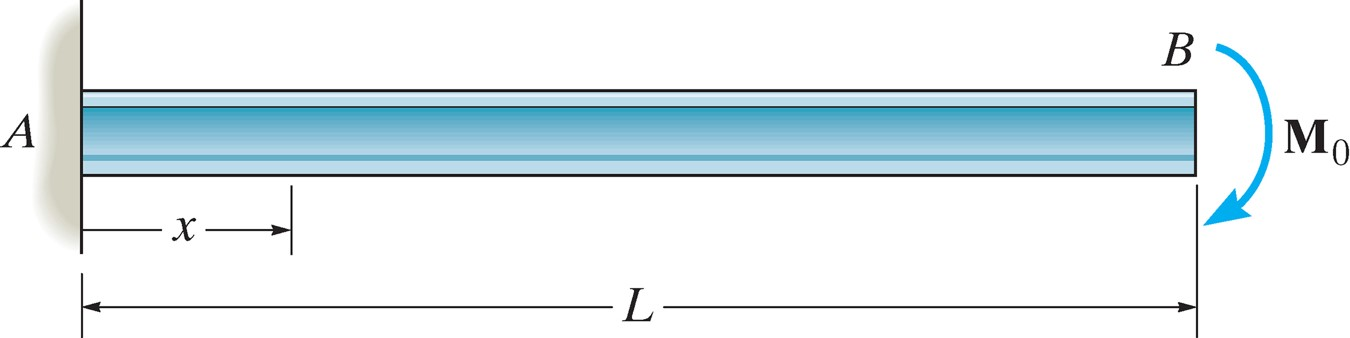
\includegraphics[width=0.6\linewidth]{12-6}
		\end{figure}
			\textbf{Solution:}
			\begin{itemize}
				\item Statics to find the reactions gives that there is only a reaction moment, equal and opposite to the applied moment.
					Taking an internal section, we find the applied moment is negative.
				\item This gives $M(x) = -M_0 = \frac{d^2 v}{dx^2}EI$
				\item Integrating twice gives $-\frac{1}{2}M_0x^2 + C_1 x + C_2 = v EI$
				\item We can now apply the boundary conditions at the fixed end, $v(0) = 0$ and $\frac{dv}{dx}(0) = 0$ to find that $C_1 = C_2 = 0$
				\item This gives the deflection as $v(x) = -\frac{M_0}{2EI}x^2$
			\end{itemize}

	\item %12-15
		A torque wrench is used to tighten the nut on a bolt.
		If the dial indicates that a torque of $ 	\US{75}{ft.lb}  $ when the bolt is fully tightened, find the force $P$ on the handle and the distance that the needle moves along the scale.
		Assume that only the section $AB$ bends and the cross section is a solid $ 	\US{0.5 }{in}  $ square with $E = 	\US{29 }{Msi} $
		\begin{figure}[H]
			\centering
			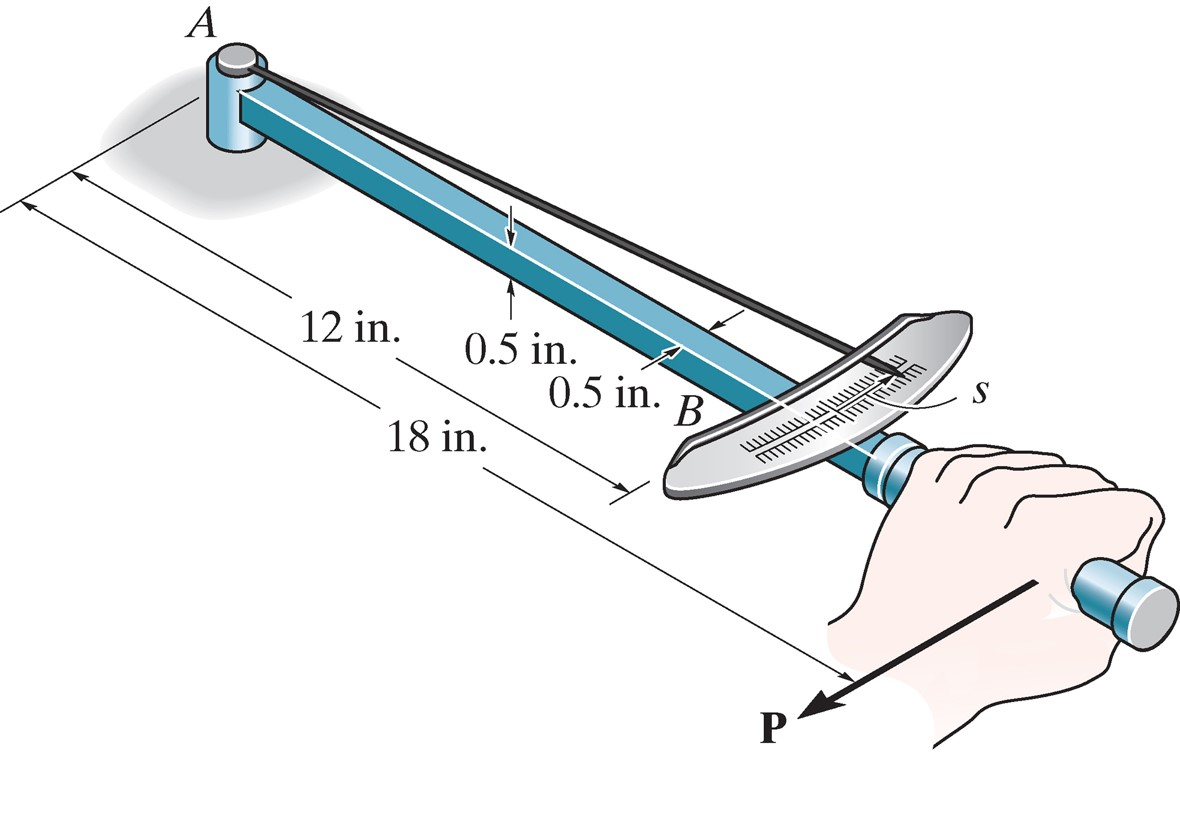
\includegraphics[width=0.6\linewidth]{12-15}
		\end{figure}
			\textbf{Solution:}
			\begin{itemize}
				\item We can consider the socket end of the wrench to be a cantilevered support. Even though it does not perfectly stop rotation like most "fixed" supports, it does resist rotation and in this case we are given the reaction moment as the torque of the bolt.
				\item We can now use statics to find the force $P$ that corresponds to the appropriate reaction moment and we find $P = 	\US{50}{lb} $
				\item We now need to section our torque wrench to find the moment as a function of $x$.
					\begin{figure}[H]
						\centering
						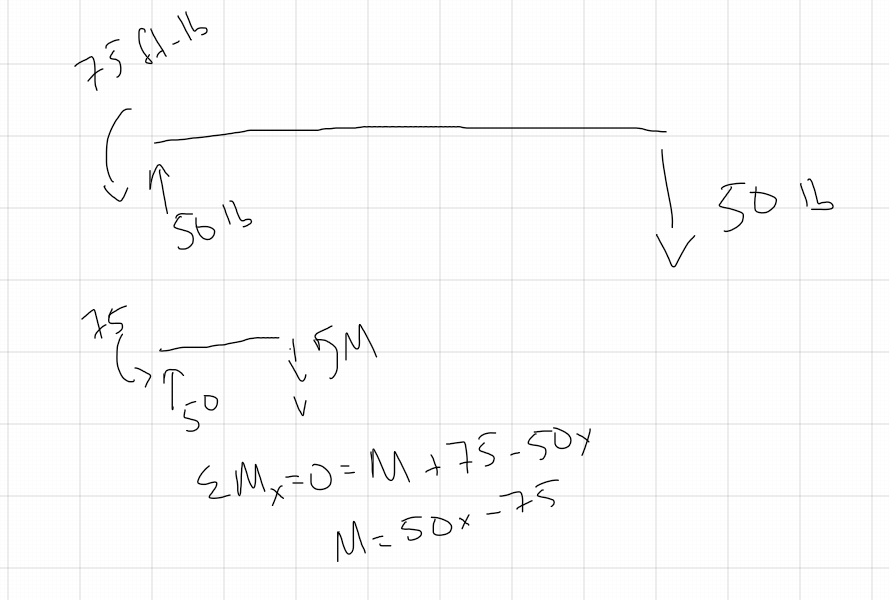
\includegraphics[width=0.6\linewidth]{12-15a}
					\end{figure}
				\item We integrate twice to find that $v EI = \frac{50}{6}x^3 - \frac{75}{2}x^2 + C_1 x + C_2$
				\item Notice that to keep consistent units, we need to use $x$ in feet, not inches (or convert $ 	\US{75}{ft lb} $ into inch-pounds), with boundary conditions of $v(0) = 0$ and $\frac{dv}{dx}(0) = 0$ we find that $C_1 = C_2 = 0$.
				\item Now we need to substitute values at $x = 	\US{12}{in} $ (and calculate the moment of inertia). At this point it is easiest to convert to inch-pounds so that our length units are consistent. We find that $I=\US{.0052}{in^4}$ and $ 	\US{75}{ft.lb} = 	\US{900}{in.lb}$ which gives $v(12) = 	\US{-0.334}{in} $
			\end{itemize}

	\item %12-25
		The floor beam of an airplane is subjected to the loading shown.
		Assuming the fuselage exerts only vertical reactions on the ends of the beam, determine the maximum deflection of the beam in terms of some constant flexural rigidity, $EI$.
		\begin{figure}[H]
			\centering
			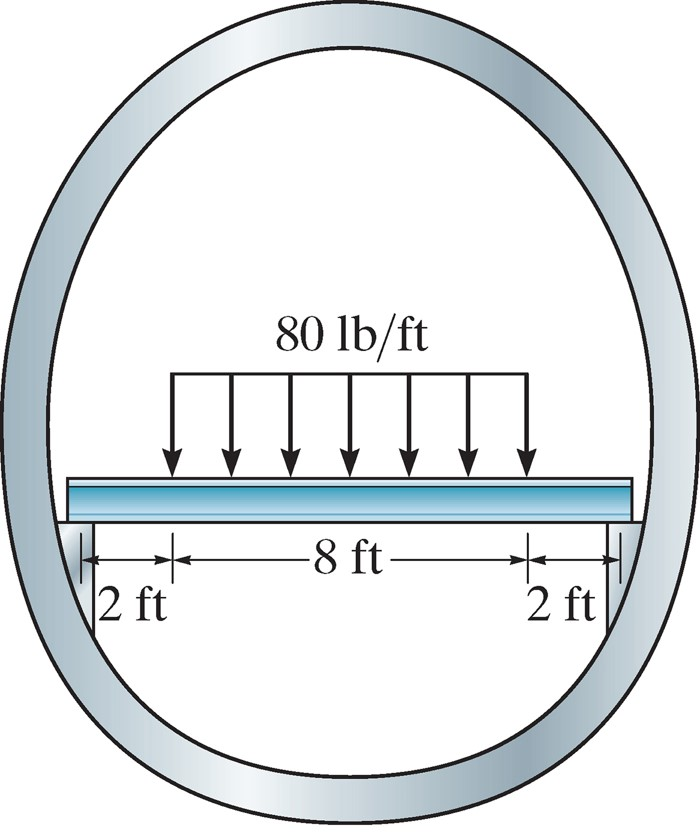
\includegraphics[width=0.6\linewidth]{12-25}
		\end{figure}
			\textbf{Solution:}
			\begin{itemize}
				\item For this problem I will use the discontinuity function approach in my solutions
				\item We have $ 	\US{80}{lb/ft}  $ acting over 8 feet, which means 640 lbs, and each reaction will be 320 lbs.
				\item This gives our moment equation as $M = 320 - 40 \langle x-2 \rangle^2 + 40 \langle x-10 \rangle^2$
				\item Integrating twice gives $v EI = 160x^2 - 10/3 \langle x-2 \rangle^4 + 10/3 \langle x-10 \rangle^4 + C_1x + C_2$
				\item We can find the unknown constants by substituting boundary conditions of $v(0) = 0$ and $v(12) = 0$.
				\item We find $C_2 = 0$ and $C_1 = 853.3$
				\item The maximum deflection, since this is symmetric, will occur at the middle, so we can substitute $x=6$ to find $v = \frac{1}{EI}(10026.7)$
			\end{itemize}

	\item %12-35
		Find the deflection as a function of $x$ for the beam shown in terms of some constant $EI$.
		\begin{figure}[H]
			\centering
			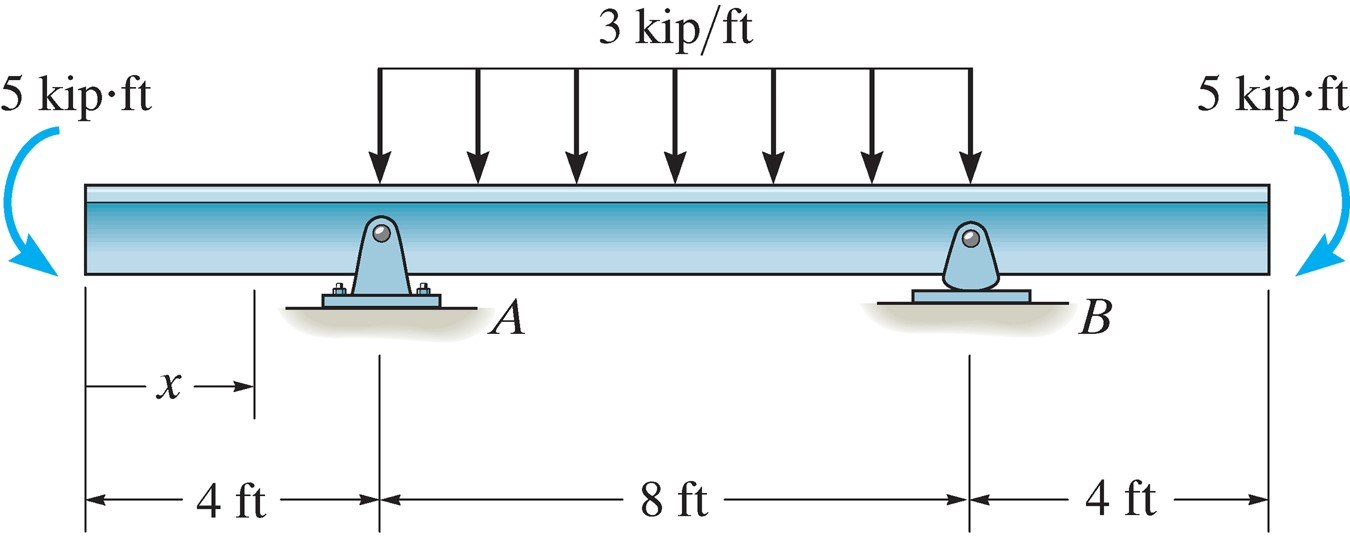
\includegraphics[width=0.6\linewidth]{12-35}
		\end{figure}
			\textbf{Solution:}
			\begin{itemize}
				\item From statics we find the reaction forces are both $ 	\US{12}{kip}  $
				\item Using the discontinuity function method, we find the moment as a function of $x$ to be $M(x) = 	\US{-5 }{kip.ft} + 	\US{12}{kip}\langle x-4 \rangle - 	\US{3/2}{kip/ft} \langle x-4 \rangle^2 + 	\US{12}{kip}\langle x-12 \rangle + 	\US{3/2}{kip}\langle x-12 \rangle^2 $
				\item Integrating twice gives $EI v(x) = -\frac{5}{2}x^2 + 	2 \langle x-4 \rangle^3 - 	\frac{1}{8}\langle x-4 \rangle^4 + 	2 \langle x-12 \rangle^3 + 	\frac{1}{8} {kip}\langle x-12 \rangle^4 + C_1 x + C_2$
				\item In this problem the boundary conditions are $v(4)=0$ and $v(12)=0$ which gives
					\begin{align*}
						0 &=  -\frac{5}{2}(4)^2 + C_1 (4) + C_2\\
						0 &= -\frac{5}{2}(12)^2 +	2(8) -\frac{1}{8}(8)^4 + C_1(12) + C_2
					\end{align*}
				\item We find $C_1 = 102$ and $C_2 = -368$ which gives the total deflection, in terms of $EI$ as
					\[ v(x) = \frac{1}{EI} \left (-\frac{5}{2}x^2 + 	2 \langle x-4 \rangle^3 - 	\frac{1}{8}\langle x-4 \rangle^4 + 	2 \langle x-12 \rangle^3 + 	\frac{1}{8} {kip}\langle x-12 \rangle^4 + 102 x - 368 \right)\]
			\end{itemize}

	\item %12-39
		Find the deflection as a function of $x$ for the beam shown in terms of some constant $EI$.
		\begin{figure}[H]
			\centering
			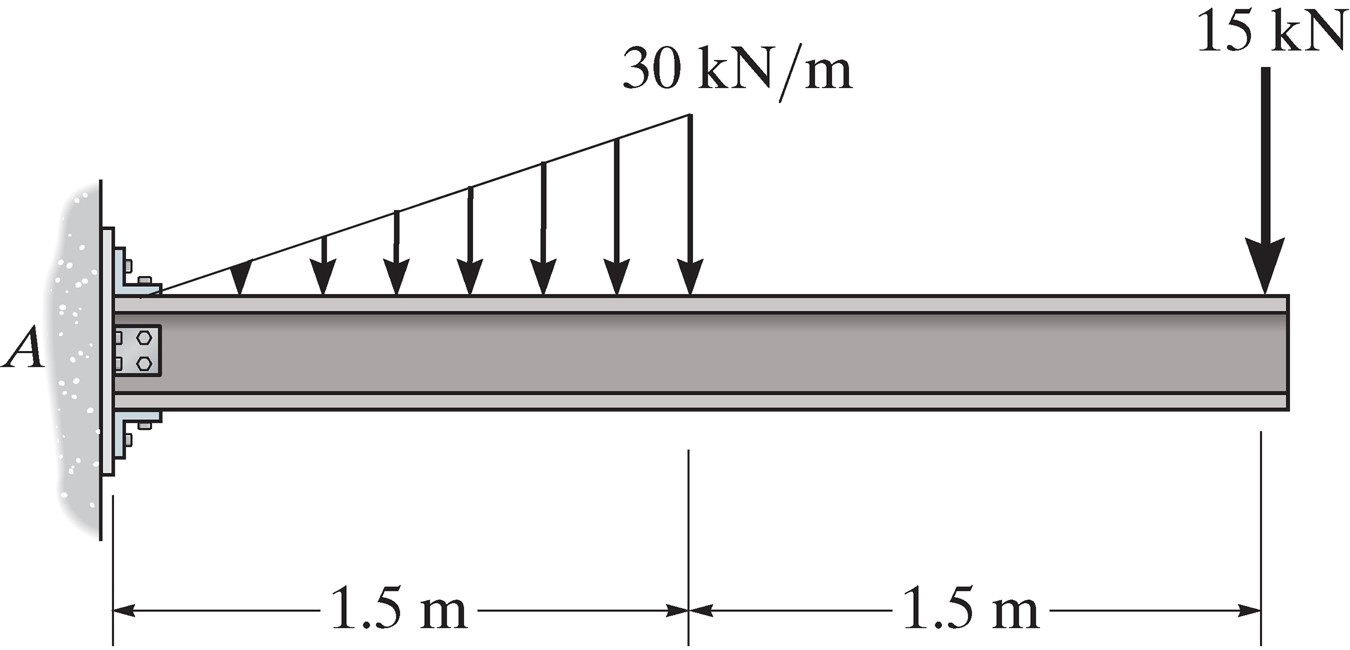
\includegraphics[width=0.6\linewidth]{12-39}
		\end{figure}
			\textbf{Solution:}
			\begin{itemize}
				\item Once again we start with statics to find the reactions. We find the vertical force at $A$ is $ 	\SI{37.5}{kN}  $ while the reaction moment is $ 	\SI{67.5}{kN.m}  $
				\item It is a bit tricky to apply the distributed load correctly, see the drawing to show the necessary superposition, starting at 0 the discontinuity function applies a linearly increasing distributed load on the entire beam, and we need both a uniform and linearly increasing distributed load to cancel it.
					\begin{figure}[H]
						\centering
						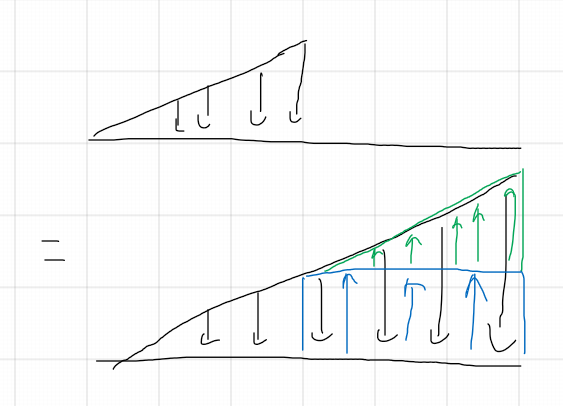
\includegraphics[width=0.6\linewidth]{12-39a}
					\end{figure}
				\item All told this gives $M(x) = 60x -90 -5x^3 + 5 \langle x-1.5\rangle^3 + \frac{45}{2} \langle x-1.5 \rangle^2$
				\item Integrating twice gives $EI v(x) = 10x^3 - 45x^2 - \frac{1}{4}x^5 - \frac{1}{4} \langle x-1.5 \rangle^5 + \frac{15}{8}\langle x-1.5 \rangle^4 + C_1 x + C_2$
				\item Applying boundary conditions of $v(0) = 0$ and $dv/dx(0) = 0$ gives $C_1 = C_2 = 2$ and our final deflection equation is $v(x) = \frac{1}{EI} \left( 10x^3 - 45x^2 - \frac{1}{4}x^5 - \frac{1}{4} \langle x-1.5 \rangle^5 + \frac{15}{8}\langle x-1.5 \rangle^4 \right)$
			\end{itemize}

	\item %12-93
		The rod is pinned at the end $A$ and attached to a torsional spring with stiffness $k$ (with $k$ expressed in torque per radian of rotation).
		For a perpendicular force, $P$, as shown find the displacement of the force in terms of some constant $EI$.
		\begin{figure}[H]
			\centering
			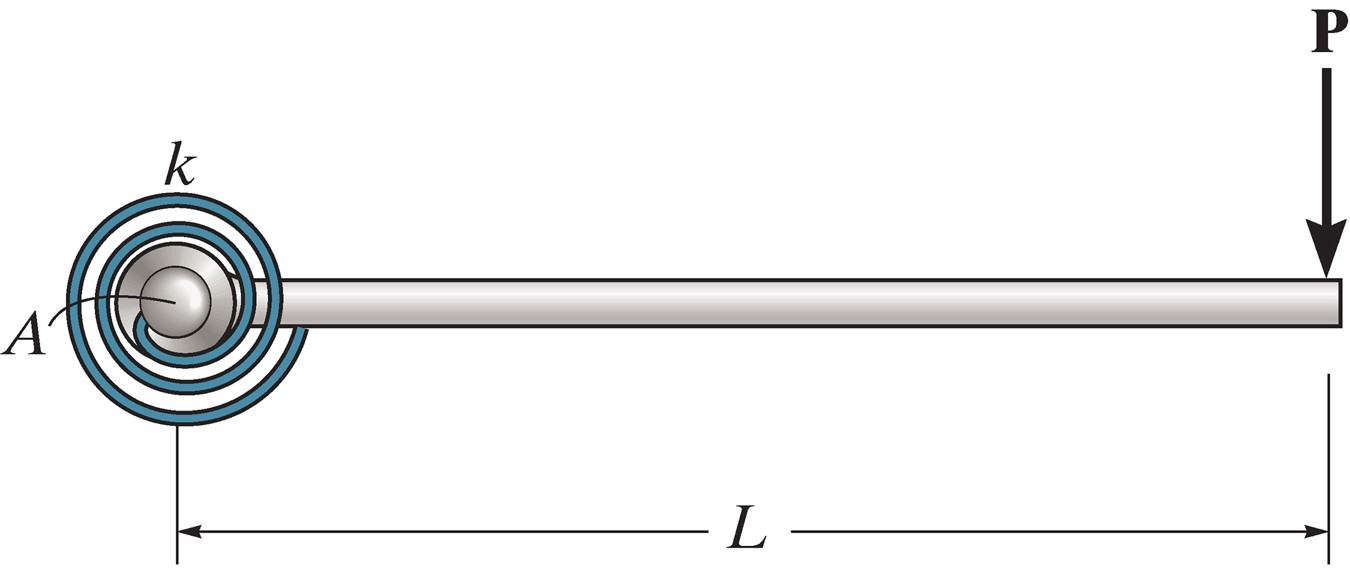
\includegraphics[width=0.6\linewidth]{12-93}
		\end{figure}
			\textbf{Solution:}
			\begin{itemize}
				\item We will use the superposition method to solve this problem.
				\item Some of the deflection will occur from the rod bending like a cantilever beam, while the rest will come from rigid rotation about the spring, we can add these two solutions together.
					\begin{figure}[H]
						\centering
						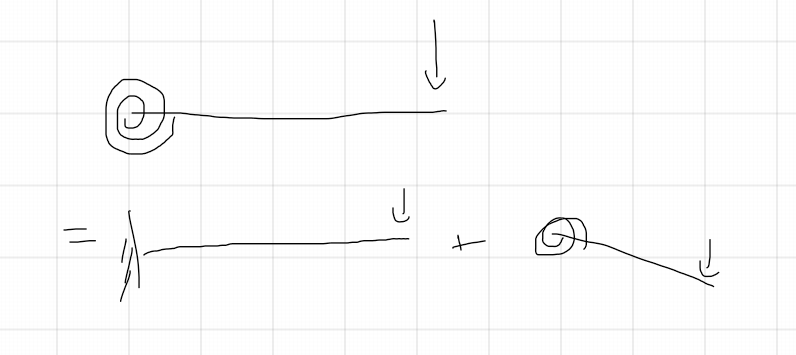
\includegraphics[width=0.6\linewidth]{12-93a}
					\end{figure}
				\item The rigid spring rotation will occur with the spring torque $k\theta$ equal to the applied moment, $PL$, we can find the angle in terms of the other parameters as $\theta = \frac{PL}{k}$. We know that $\tan \theta = \frac{v_1}{L}$, so we can say that $v_1 = -L \tan \frac{PL}{k}$ (negative sign added to indicate that deflection goes down).
				\item The cantilever portion we can obtain directly from Appendix C, where we find  $v_2 = -\frac{Px^2}{6EI}(3L - x)$
				\item We add the two solutions to find the total deflection $v = v_1 + v_2 =  -L \tan \frac{PL}{k} -\frac{Px^2}{6EI}(3L - x)$
			\end{itemize}

\end{enumerate}
\end{document}
